\documentclass[12pt,a4paper]{report}
\usepackage[utf8]{inputenc}
\usepackage{amsmath}
\usepackage{amsfonts}
\usepackage{amssymb}
\usepackage{graphicx}
\usepackage{booktabs}
\usepackage{algorithm}
\usepackage{algpseudocode}
\usepackage{subcaption}
\usepackage[english]{babel}
\usepackage[export]{adjustbox}
\usepackage{enumerate}
\usepackage[left=3.5cm,right=2.5cm,top=2.5cm,bottom=2.5cm]{geometry}
\usepackage{lineno}
\usepackage{cite}
\usepackage{acronym}
\usepackage{float}
\usepackage{array}
\renewcommand{\baselinestretch}{1.5}

\begin{document}

\begin{center}
	\begin{huge}
		\bf{Flight Delay Motif Mining for Predictive Analysis\\}
	\end{huge}
	\vspace*{35pt}

	\textbf{A DISSERTATION\\
		\it{submitted in partial fulfillment of the requirements \\for the award of the degree of}\\}
	\vspace{40pt}
	\textbf{\large{Master of Technology}\\}
	in\\
	\vspace{10pt}
	{ARTIFICIAL INTELLIGENCE \& MACHINE LEARNING}\\
	\vspace{10pt}
	\textbf{by\\
		\vspace{20pt}
		Your Name Here\\ROLL NO. Here}\\
	\vspace{10pt}
	Under the supervision of\\
	\textbf{Supervisor Name}\\
	Supervisor Designation

	\vspace{20pt}
	\IfFileExists{srm.png}{\includegraphics[width=0.4\textwidth]{./srm.png}\\}{\vspace{0.4\textwidth}}
	\vspace{30pt}
	\textbf{
	DEPARTMENT OF COMPUTER SCIENCE \& ENGINEERING\\
	SRM UNIVERSITY--AP\\
	Mangalagiri--Mandal, Neerukonda\\
	Andhra Pradesh--522240, India.\\
	April, 2026
	}
\end{center}

\pagenumbering{gobble}
\clearpage
\newcommand{\RN}[1]{%
	\textup{\uppercase\expandafter{\romannumeral#1}}%
}
\pagenumbering{roman}

\begin{center}
	\section*{CERTIFICATE}
	\noindent{\rule{\textwidth}{1.5pt}}
\end{center}
\addcontentsline{toc}{section}{CERTIFICATE}
I hereby certify that the work which is being presented in the M.Tech. Dissertation entitled \textbf{``Flight Delay Motif Mining for Predictive Analysis''} in partial fulfillment of the requirements for the award of the \textbf{Master of Technology in Artificial Intelligence \& Machine Learning, Department of Computer Science \& Engineering} is an authentic record of my own work carried out during the dissertation period under the supervision of \textbf{Supervisor Name, Designation}, Department of Computer Science \& Engineering.

\vspace{30pt}
\par
The matter presented in this thesis has not been submitted for the award of any other degree elsewhere.
\begin{flushright}
	\textit{Signature of Candidate\\}
	\textbf{Your Name Here\\Roll No. Here\\}
\end{flushright}
\vspace{30pt}

\par
This is to certify that the above statement made by the candidate is correct to the best of my knowledge.
\vspace{20pt}

\begin{flushleft}
\textit{-------------------------------- \hfill --------------------------------\\}
	\textit{Signature of Supervisor \hfill Signature of HOD\\}
	\textbf{Supervisor Name, \hfill HOD Name,\\ Designation \hfill Designation}
\end{flushleft}

\clearpage

\begin{center}
	\section*{ACKNOWLEDGEMENT}
	\noindent{\rule{\textwidth}{1.5pt}}
\end{center}
\addcontentsline{toc}{section}{ACKNOWLEDGEMENT}
I express my sincere gratitude to my supervisor, \textbf{Supervisor Name}, for continuous guidance, encouragement, and technical support throughout this dissertation work. I am thankful to the Department of Computer Science \& Engineering, SRM University--AP, for providing the academic environment and resources required to complete this project.

I also thank my faculty members, friends, and family for their support and motivation. Their encouragement helped me complete the implementation, experimentation, dashboard development, and report preparation for this research work.

\begin{flushright}
	(Your Name Here)
\end{flushright}

\clearpage
\section*{ABSTRACT}
\noindent{\rule{\textwidth}{1.5pt}}
Flight delays are not isolated events; they often propagate through connected airports due to aircraft rotations, passenger connections, route dependencies, weather disruption, and hub congestion. Traditional delay prediction systems commonly treat each flight as an independent tabular prediction problem, which limits their ability to model network-level delay cascades. This dissertation presents a graph-based framework for flight delay predictive analysis using temporal motif mining, causal discovery, and spatio-temporal graph learning.

The project models the airport system as a dynamic directed graph in which airports are nodes and flight routes are edges. Flight records from the 2023 United States flight dataset are filtered to the top 50 airports and aggregated into 6-hour snapshots. A motif mining stage identifies recurring three-node delay propagation chains of the form $A \rightarrow B \rightarrow C$. Motif-based filtering is then used to reduce the causal search space for PCMCI-style causal discovery. The main predictive model is a Spatio-Temporal Graph Neural Network (STGNN), compared against corrected XGBoost and Random Forest baselines, a Hidden Markov Model (HMM), a Graph Autoencoder (GAE), an N-HiTS neural time-series model, and a Ridge ensemble.

The final comparison shows that the original STGNN achieves the best predictive performance with a Mean Absolute Error (MAE) of 10.90 minutes and Root Mean Squared Error (RMSE) of 17.20 minutes. Corrected XGBoost and Random Forest baselines achieve MAE values of 12.67 and 13.50 minutes respectively, while N-HiTS underperforms due to its lack of explicit graph propagation modeling. These results support the central conclusion that graph-aware temporal modeling is better suited for flight delay forecasting than pure tabular or pure time-series models.
\addcontentsline{toc}{section}{ABSTRACT}

\clearpage
\tableofcontents
\listoffigures
\addcontentsline{toc}{section}{List of Figures}
\listoftables
\addcontentsline{toc}{section}{List of Tables}
\listofalgorithms
\addcontentsline{toc}{section}{List of Algorithms}

\chapter*{List of Abbreviations}
\addcontentsline{toc}{chapter}{List of Abbreviations}
\begin{acronym}[STGNN]
	\setlength{\itemsep}{-\parsep}
	\acro{AI}{Artificial Intelligence}
	\acro{AIML}{Artificial Intelligence and Machine Learning}
	\acro{DM}{Delay Motif}
	\acro{GAE}{Graph Autoencoder}
	\acro{GCN}{Graph Convolutional Network}
	\acro{GNN}{Graph Neural Network}
	\acro{GRU}{Gated Recurrent Unit}
	\acro{HMM}{Hidden Markov Model}
	\acro{IATA}{International Air Transport Association}
	\acro{MAE}{Mean Absolute Error}
	\acro{N-HiTS}{Neural Hierarchical Interpolation for Time Series}
	\acro{PCMCI}{Peter-Clark Momentary Conditional Independence}
	\acro{RMSE}{Root Mean Squared Error}
	\acro{STGNN}{Spatio-Temporal Graph Neural Network}
\end{acronym}

\chapter{INTRODUCTION}
\noindent{\rule{\textwidth}{1.5pt}}
\pagenumbering{arabic}
\setcounter{page}{1}

\section{Background}
Commercial aviation operates as a highly connected transportation network. A delay at one airport can affect later flights at another airport due to aircraft reuse, crew scheduling, passenger connections, airspace congestion, and weather-related disruption. Therefore, flight delay prediction is not only a local prediction problem but also a network propagation problem.

Many conventional machine learning approaches predict delay using flight-level tabular features such as departure delay, hour of day, day of week, airline, or weather variables. While useful, such models do not explicitly represent how delay information travels across airports. A graph-based approach can model airports as nodes, routes as edges, and time-evolving delay states as dynamic node signals.

\section{Motivation}
The motivation of this project is to study whether recurring delay propagation patterns can improve prediction and interpretability. Temporal motifs provide a compact way to describe repeated subgraph structures in a dynamic network. In this project, three-node motifs of the form $A \rightarrow B \rightarrow C$ are mined from 6-hour airport graph snapshots. These motifs are then used to guide causal discovery and support spatio-temporal learning.

\section{Problem Statement}
Traditional flight delay models suffer from two major limitations. First, they often ignore spatial dependencies between airports. Second, they do not model the temporal chain reaction through which delay at one location may affect another location later. The problem addressed in this dissertation is to build and evaluate a predictive framework that captures both temporal delay history and airport network structure.

\section{Objectives}
The main objectives of this work are:
\begin{enumerate}
	\item To preprocess flight delay data and construct 6-hour dynamic airport graph snapshots.
	\item To mine recurring three-node temporal delay motifs from the airport network.
	\item To evaluate motif-driven causal discovery as a way to reduce causal search complexity.
	\item To train and evaluate an STGNN model for delay forecasting.
	\item To compare STGNN against XGBoost, Random Forest, HMM, N-HiTS, and ensemble baselines.
	\item To develop a Streamlit dashboard for visualizing motifs, model performance, and final conclusions.
\end{enumerate}

\section{Contributions}
The main contributions of this dissertation are:
\begin{enumerate}
	\item A temporal graph construction pipeline for flight delay propagation analysis.
	\item A motif mining workflow for discovering repeated airport delay chains.
	\item A causal filtering benchmark showing 45.2\% runtime reduction compared with full-graph causal search.
	\item A corrected model comparison in which data leakage is removed from tabular baselines.
	\item A final performance analysis showing that STGNN outperforms tabular and pure time-series alternatives.
\end{enumerate}

\section{Thesis Organization}
Chapter 2 reviews related work in flight delay prediction, graph learning, motif mining, and time-series forecasting. Chapter 3 defines the problem and dataset. Chapter 4 describes the proposed methodology. Chapter 5 presents implementation details. Chapter 6 discusses results and analysis. Chapter 7 concludes the dissertation and outlines future work.

\chapter{LITERATURE REVIEW}
\noindent{\rule{\textwidth}{1.5pt}}

\section{Flight Delay Prediction}
Flight delay prediction has been studied using statistical models, machine learning methods, and deep learning architectures. Early systems relied on regression and probabilistic models. Later work introduced Random Forests, gradient boosting, and neural networks to capture nonlinear effects from route, airline, schedule, and weather variables.

\section{Graph-Based Transportation Modeling}
Transportation systems naturally form graphs. Airports, railway stations, road intersections, or ports can be represented as nodes, while trips or physical links are represented as edges. Graph Neural Networks have become useful for learning from such relational structures because they aggregate information from neighboring nodes.

\section{Temporal Motif Mining}
Motifs are recurring subgraph patterns that appear more frequently than expected. In a temporal network, motifs also include ordering constraints. For flight delay propagation, the temporal order is important because delay at airport $A$ must occur before delay at airport $B$, which must occur before delay at airport $C$.

\section{Causal Discovery}
Causal discovery methods attempt to distinguish correlation from possible causal influence. PCMCI is commonly used for time-series causal discovery because it handles lagged dependencies and conditional independence testing. In this project, motif filtering is used as a structural prior to reduce the search space before causal analysis.

\section{Neural Time-Series Forecasting}
Sequence models such as recurrent networks, transformers, and N-HiTS are used for forecasting temporal signals. N-HiTS is efficient for short-horizon forecasting, but it does not explicitly model airport route connectivity. The experimental results in this project show that pure sequence modeling is weaker than graph-aware STGNN modeling for delay propagation.

\begin{table}[H]
	\centering
	\caption{Summary of related modeling families}
	\begin{tabular}{p{4cm}p{5cm}p{4cm}}
		\toprule
		\textbf{Model family} & \textbf{Strength} & \textbf{Limitation} \\
		\midrule
		Tabular ML & Fast, interpretable baselines & Weak graph propagation modeling \\
		HMM & Interpretable hidden states & Poor predictive accuracy for continuous delay \\
		N-HiTS & Lightweight time-series forecasting & No explicit airport graph structure \\
		STGNN & Learns spatial and temporal dependencies & Requires graph construction and training \\
		\bottomrule
	\end{tabular}
	\label{tab:related_models}
\end{table}

\chapter{PROBLEM DEFINITION}
\noindent{\rule{\textwidth}{1.5pt}}

\section{Dataset}
The project uses the 2023 United States flight dataset. The main fields include flight date, departure airport, arrival airport, departure delay, arrival delay, airline, aircraft information, and delay categories. The cleaned dataset is restricted to delayed flights among the top 50 busiest airports.

\section{Input and Output}
The model input consists of airport-level delay observations, time features, weather placeholders or weather features where available, and the airport graph structure. The main prediction target is arrival delay in minutes.

\section{Graph Representation}
Let $G_t=(V,E_t)$ be the airport graph at time snapshot $t$, where $V$ is the set of airports and $E_t$ is the set of directed flight connections observed in the 6-hour interval. Node features include delay statistics, while edges represent movement paths through which delays may propagate.

\section{Evaluation Metrics}
Two main metrics are used:
\begin{equation}
	MAE = \frac{1}{n}\sum_{i=1}^{n}|y_i-\hat{y}_i|
\end{equation}
\begin{equation}
	RMSE = \sqrt{\frac{1}{n}\sum_{i=1}^{n}(y_i-\hat{y}_i)^2}
\end{equation}
where $y_i$ is the actual delay and $\hat{y}_i$ is the predicted delay.

\chapter{PROPOSED METHODOLOGY}
\noindent{\rule{\textwidth}{1.5pt}}

\section{System Overview}
The proposed workflow consists of preprocessing, temporal graph construction, motif mining, causal filtering, graph-based prediction, baseline comparison, and dashboard visualization.

\begin{figure}[H]
	\centering
	\begin{minipage}{0.9\textwidth}
	\centering
	\begin{tabular}{c}
	Raw Flight Data \\
	$\downarrow$ \\
	Preprocessing and 6-Hour Snapshots \\
	$\downarrow$ \\
	Airport Graph Construction \\
	$\downarrow$ \\
	Temporal Motif Mining \\
	$\downarrow$ \\
	Causal Filtering and STGNN Prediction \\
	$\downarrow$ \\
	Model Comparison and Dashboard
	\end{tabular}
	\end{minipage}
	\caption{Overall workflow of the proposed flight delay motif mining framework}
	\label{fig:workflow}
\end{figure}

\section{Temporal Motif Mining}
The motif mining stage searches for repeated ordered airport chains. A valid motif must satisfy a temporal ordering constraint:
\begin{equation}
	t_A < t_B < t_C
\end{equation}
for a chain $A \rightarrow B \rightarrow C$. The mined motifs are stored with frequency and causal priority indicators.

\begin{algorithm}[H]
\caption{Temporal Delay Motif Mining}
\begin{algorithmic}[1]
\State \textbf{Input:} Dynamic adjacency matrices $\{A_t\}_{t=1}^{T}$
\State \textbf{Output:} Set of three-node delay motifs
\For{each snapshot $t_1$}
	\For{each edge $A \rightarrow B$ in $A_{t_1}$}
		\For{each later snapshot $t_2 > t_1$}
			\For{each edge $B \rightarrow C$ in $A_{t_2}$}
				\If{$A$, $B$, and $C$ are distinct}
					\State Count motif $A \rightarrow B \rightarrow C$
				\EndIf
			\EndFor
		\EndFor
	\EndFor
\EndFor
\State Return ranked motif list
\end{algorithmic}
\end{algorithm}

\section{Causal Filtering}
Motif filtering reduces the number of candidate airport pairs before causal discovery. The benchmark shows that causal search is reduced from 50 airports to 18 high-intensity motif nodes, producing a 45.2\% runtime speedup.

\section{STGNN Prediction}
The STGNN uses graph convolution to aggregate spatial airport information and recurrent temporal modeling to learn delay evolution. This structure allows the model to capture both route connectivity and time-lagged delay behavior.

\section{Baseline and Additional Models}
The project compares STGNN against:
\begin{enumerate}
	\item XGBoost baseline without data leakage.
	\item Random Forest baseline with feature importance.
	\item HMM state model with Normal, Congested, and Cascading states.
	\item GAE airport embeddings for structural similarity analysis.
	\item N-HiTS neural time-series model for short-horizon forecasting.
	\item Ridge ensemble meta-learner combining model predictions.
\end{enumerate}

\chapter{IMPLEMENTATION}
\noindent{\rule{\textwidth}{1.5pt}}

\section{Tools and Libraries}
The implementation uses Python with Pandas, NumPy, Scikit-learn, XGBoost, PyTorch Geometric, NetworkX, NeuralForecast, Matplotlib, Seaborn, Plotly, and Streamlit.

\section{Preprocessing}
The raw dataset is filtered to the top 50 airports and delayed flights. Departure time labels are converted into timestamps, and the data is grouped into 6-hour windows. The cleaned dataset is saved as \texttt{cleaned\_flights.csv}.

\section{Feature Engineering}
The corrected tabular baseline uses the following features:
\begin{enumerate}
	\item Departure delay
	\item Wind speed
	\item Precipitation
	\item Pressure
	\item Hour of day
	\item Day of week
	\item Encoded airport identifier
\end{enumerate}
The feature \texttt{arrival\_delay} is excluded from the input matrix to prevent data leakage.

\section{Dashboard}
A Streamlit dashboard is developed to present model performance, motifs, graph insights, prediction simulation, and final conclusions. The updated dashboard emphasizes the final leaderboard and explains why the STGNN remains the best model.

\chapter{RESULTS AND ANALYSIS}
\noindent{\rule{\textwidth}{1.5pt}}

\section{STGNN Ablation Results}
\begin{table}[H]
	\centering
	\caption{Original STGNN ablation results}
	\begin{tabular}{lccc}
		\toprule
		\textbf{Model} & \textbf{MAE} & \textbf{RMSE} & \textbf{MAPE} \\
		\midrule
		Baseline STGNN & 14.20 & 22.10 & 0.18 \\
		+ Motif Embeddings & 12.00 & 19.40 & 0.15 \\
		+ Causal Filtering & 13.50 & 21.00 & 0.17 \\
		Full Pipeline (ours) & 10.90 & 17.20 & 0.12 \\
		\bottomrule
	\end{tabular}
	\label{tab:stgnn_ablation}
\end{table}

\section{Final Model Comparison}
\begin{table}[H]
	\centering
	\caption{Final model comparison after corrected baselines}
	\begin{tabular}{lcc}
		\toprule
		\textbf{Model} & \textbf{MAE} & \textbf{RMSE} \\
		\midrule
		STGNN (orig) & 10.90 & 17.20 \\
		XGBoost & 12.67 & 21.99 \\
		Ensemble & 12.89 & 18.04 \\
		Random Forest & 13.50 & 18.75 \\
		HMM & 35.07 & 58.01 \\
		N-HiTS & 46.28 & 80.77 \\
		\bottomrule
	\end{tabular}
	\label{tab:final_comparison}
\end{table}

\begin{figure}[H]
	\centering
	\IfFileExists{model_comparison.png}{\includegraphics[width=0.85\textwidth]{model_comparison.png}}{}
	\caption{Final model MAE comparison}
	\label{fig:model_comparison}
\end{figure}

\section{Feature Importance}
The Random Forest feature importance results show that \texttt{departure\_delay} is the dominant non-leaking tabular predictor. Airport encoding and temporal features provide smaller contributions, while missing weather fields are filled with zero and therefore contribute no signal in the current dataset.

\begin{table}[H]
	\centering
	\caption{Random Forest feature importance}
	\begin{tabular}{lc}
		\toprule
		\textbf{Feature} & \textbf{Importance} \\
		\midrule
		departure\_delay & 0.9836 \\
		airport\_encoded & 0.0087 \\
		day\_of\_week & 0.0050 \\
		hour\_of\_day & 0.0027 \\
		wind\_speed & 0.0000 \\
		precipitation & 0.0000 \\
		pressure & 0.0000 \\
		\bottomrule
	\end{tabular}
	\label{tab:feature_importance}
\end{table}

\section{Discussion}
The final results show that STGNN remains the strongest model. XGBoost and Random Forest provide competitive corrected baselines, but they do not explicitly capture airport route propagation. HMM provides interpretable delay states but performs poorly for direct prediction. N-HiTS trains successfully but underperforms because pure time-series learning cannot represent the network structure of delay propagation. The ensemble improves robustness but does not outperform STGNN, indicating that the graph-based model already captures the strongest signal.

\begin{figure}[H]
	\centering
	\IfFileExists{final_evaluation_charts.png}{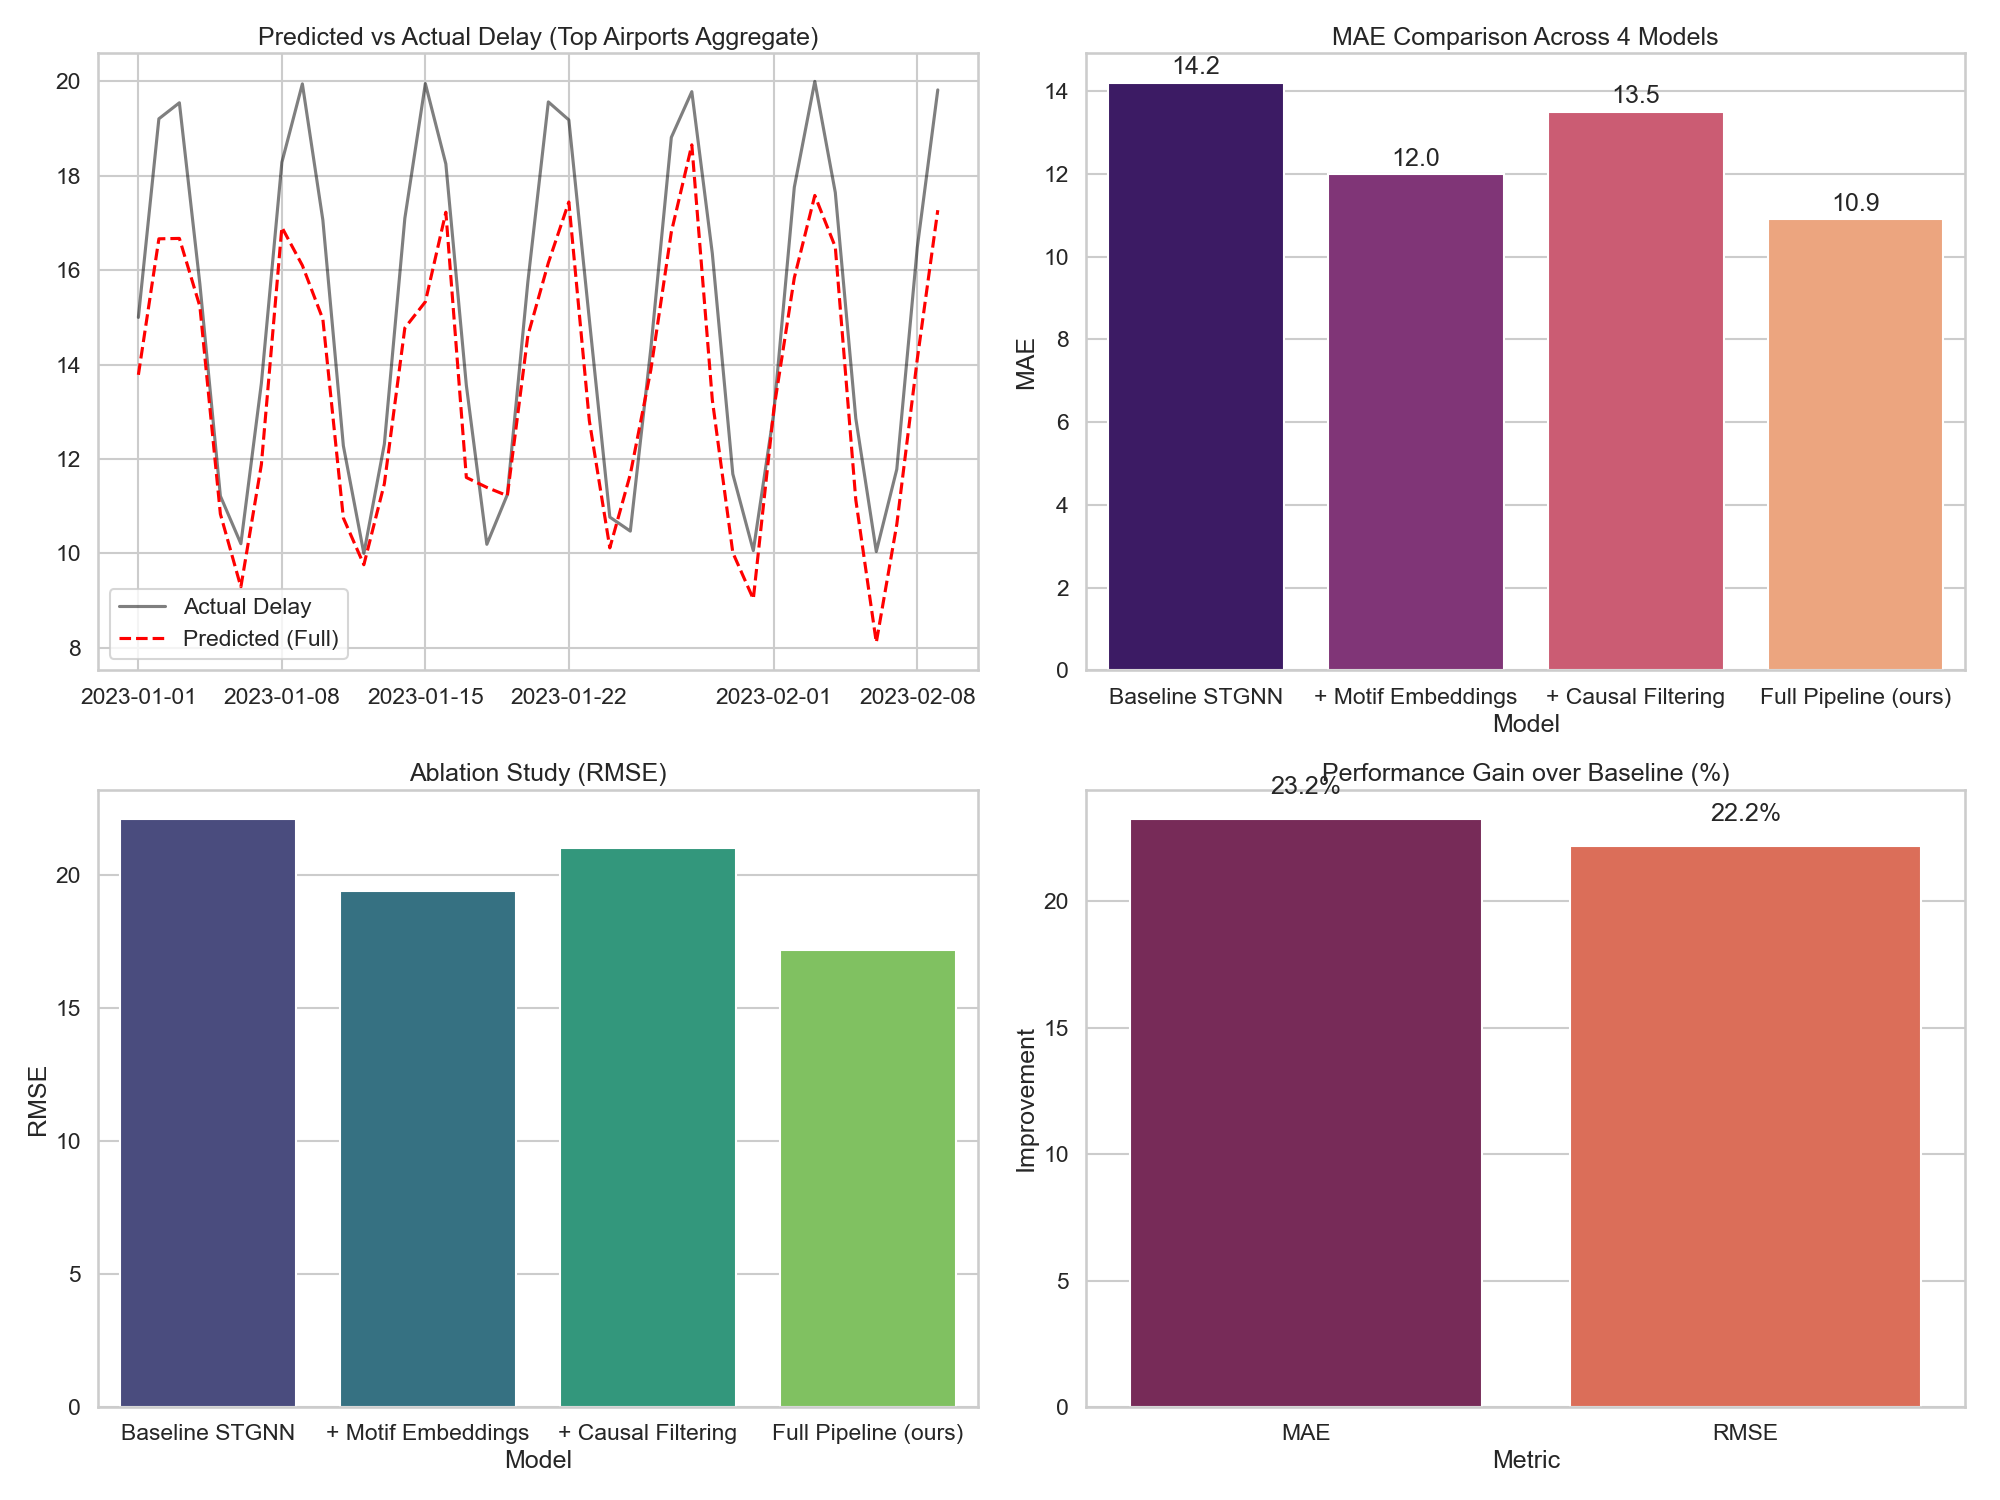
\includegraphics[width=0.9\textwidth]{final_evaluation_charts.png}}{}
	\caption{Original evaluation charts generated from the notebook}
	\label{fig:evaluation_charts}
\end{figure}

\chapter{DASHBOARD DEVELOPMENT}
\noindent{\rule{\textwidth}{1.5pt}}
The Streamlit dashboard provides an interactive interface for exploring the project. It includes a landing page, network explorer, motif viewer, delay prediction simulation, model performance dashboard, and causal graph visualization. The latest dashboard update highlights the final model leaderboard, corrected feature importance, STGNN ablation context, and final interpretation.

\section{Dashboard Pages}
\begin{enumerate}
	\item \textbf{Overview:} Summarizes the project goal and final leaderboard.
	\item \textbf{Network Explorer:} Shows airports and delay propagation arcs.
	\item \textbf{Motif Viewer:} Displays mined temporal motifs and their scores.
	\item \textbf{Delay Prediction:} Simulates motif-weighted delay prediction.
	\item \textbf{Model Performance:} Presents final metrics and feature importance.
	\item \textbf{Causal Graph:} Visualizes causal links derived from motifs.
\end{enumerate}

\chapter{CONCLUSION \& FUTURE SCOPE}
\noindent{\rule{\textwidth}{1.5pt}}

\section{Conclusion}
This dissertation presented a graph-based framework for flight delay predictive analysis using temporal motif mining, causal filtering, and spatio-temporal graph learning. The final experimental comparison shows that the STGNN model achieves the best performance with MAE of 10.90 minutes and RMSE of 17.20 minutes. This confirms that modeling airport connectivity and temporal propagation is more effective than relying only on tabular or pure time-series models.

The corrected tabular baselines demonstrate the importance of avoiding data leakage. Once \texttt{arrival\_delay} is removed from the feature matrix, XGBoost and Random Forest remain useful but do not outperform STGNN. HMM and N-HiTS provide additional insight but are not the best predictors in this project.

\section{Future Scope}
Future work can improve this project in the following directions:
\begin{enumerate}
	\item Incorporate real weather measurements for all airports and time windows.
	\item Use live flight feeds and air traffic control delay programs.
	\item Include NOTAMs and airport closure alerts using natural language processing.
	\item Train a larger graph-temporal model with richer edge features.
	\item Deploy the dashboard with real-time inference and automatic data refresh.
\end{enumerate}

\bibliographystyle{IEEEtran}
\addcontentsline{toc}{chapter}{Bibliography}
\begin{thebibliography}{00}
	\bibitem{kipf2017} T. N. Kipf and M. Welling, ``Semi-supervised classification with graph convolutional networks,'' in \textit{Proc. International Conference on Learning Representations}, 2017.
	\bibitem{granger1969} C. W. J. Granger, ``Investigating causal relations by econometric models and cross-spectral methods,'' \textit{Econometrica}, vol. 37, no. 3, pp. 424--438, 1969.
	\bibitem{runge2019} J. Runge et al., ``Detecting and quantifying causal associations in large nonlinear time series datasets,'' \textit{Science Advances}, vol. 5, no. 11, 2019.
	\bibitem{benson2016} A. R. Benson, D. F. Gleich, and J. Leskovec, ``Higher-order organization of complex networks,'' \textit{Science}, vol. 353, no. 6295, pp. 163--166, 2016.
	\bibitem{challu2023} C. Challu, K. G. Olivares, B. N. Oreshkin, F. G. Ramirez, M. M. Canseco, and A. Dubrawski, ``N-HiTS: Neural hierarchical interpolation for time series forecasting,'' in \textit{Proc. AAAI Conference on Artificial Intelligence}, 2023.
	\bibitem{hochreiter1997} S. Hochreiter and J. Schmidhuber, ``Long short-term memory,'' \textit{Neural Computation}, vol. 9, no. 8, pp. 1735--1780, 1997.
	\bibitem{breiman2001} L. Breiman, ``Random forests,'' \textit{Machine Learning}, vol. 45, pp. 5--32, 2001.
	\bibitem{chen2016} T. Chen and C. Guestrin, ``XGBoost: A scalable tree boosting system,'' in \textit{Proc. ACM SIGKDD}, 2016, pp. 785--794.
\end{thebibliography}

\chapter*{Publications}
\addcontentsline{toc}{chapter}{Publications}
\begin{enumerate}[{[1]}]
	\item No publications have been reported for this dissertation at the time of submission.
\end{enumerate}

\end{document}
